% Copyright 2026 Sreeram Anil
% SPDX-License-Identifier: CC-BY-4.0
% =============================================================================
%  Sage--Husa adaptive extended Kalman filter
% =============================================================================
\chapter{Sage--Husa adaptive extended Kalman filter (SageHusa-AKF)}
\label{ch:sagehusaakf}

\section*{At a glance}
\begin{tabular}{@{}l>{\raggedright\arraybackslash}p{0.76\textwidth}@{}}
Family & Adaptive Kalman \\
Header & \texttt{include/estkit/filters/sage\_husa\_akf.hpp} \\
Registered name & \texttt{SageHusa-AKF} \\
State dimension & $n_x = 4$ (cell model) --- generic in $n_x, n_u, n_y$ \\
Cost per step & $\mathcal{O}(n_x^3)$, EKF $+\,\mathcal{O}(n_y^2 n_x)$; $\approx 545$\,ns/step measured, no heap \\
Primary references & \cite{sagehusa1969,sagemelsa1971,maybeck1979,jazwinski1970} \\
\end{tabular}

\section{Motivation and aerospace/BMS relevance}
The Kalman filter is optimal only when the noise covariances $\mQ$ and $\mR$ that it is given are
the ones that actually generated the data.  In a battery-management system neither is known.  The
measurement-noise covariance $\mR$ is dominated by the voltage front end, whose effective noise
changes with temperature, with the switching state of the power stage, and --- in a flight vehicle
--- with the electromagnetic environment: an inverter commutating at high power can raise the
apparent voltage noise of a cell-sense channel by an order of magnitude within one flight phase.
A filter tuned for the quiet ground-test value of $\sigma_v$ then trusts a noisy measurement far
too much: its innovations become inconsistent with its own covariance, the state estimates chase
sensor noise, and any innovation-based fault monitor downstream (a standard element of a DO-178/
DO-254 class health-management chain, cf.\ the environmental qualification philosophy of
\cite{rtca2017do311a}) raises spurious alarms.

Sage and Husa \cite{sagehusa1969} were the first to give a \emph{recursive} answer: treat the
unknown noise statistics as parameters, write down the maximum-a-posteriori (MAP) estimate of those
parameters given the data seen so far, and evaluate it with an exponentially weighted (forgetting)
average so that the resulting estimator can track slow changes.  The method is attractive for
embedded use precisely because the result is a one-line recursion that re-uses quantities the
Kalman filter already computes --- the innovation, the residual and the updated covariance --- and
adds no matrix inversion and no storage beyond one $n_y\times n_y$ matrix.

The price is that the same derivation applied to the process-noise covariance $\mQ$ produces a
recursion whose increment is a \emph{difference} of covariances, and which therefore loses positive
definiteness in practice.  This chapter implements the $\mR$ recursion in its positive-definite
(residual) form as the default, keeps the $\mQ$ recursion available but disabled, and explains why.

\section{Problem statement and assumptions}
The plant is the usual discrete-time nonlinear model of \cref{ch:ecm},
\begin{align}
\vx_{k} &= f(\vx_{k-1}, \vu_{k-1}) + \vw_{k-1}, & \vw_k &\sim \N{\bm{0}}{\mQ_k}, \label{eq:sh:proc}\\
\vy_{k} &= h(\vx_{k}, \vu_{k}) + \vv_{k},       & \vv_k &\sim \N{\bm{0}}{\mR_k}, \label{eq:sh:meas}
\end{align}
where $\vx_k\in\real^{n_x}$ is the state, $\vu_k\in\real^{n_u}$ the (known) input, $\vy_k\in\real^{n_y}$
the measurement, and $\vw_k, \vv_k$ are mutually independent zero-mean white sequences.  The
functions $f$ and $h$ are known; $\mR_k$ is \emph{not}.  We assume

\begin{assumption}\label{as:sh:slow}
$\mR_k$ is constant over a window of length $\tau_R = 1/(1-b)$ samples, $b\in(0,1)$, but may change
between such windows.  Equivalently, $\mR$ is a slowly varying deterministic sequence compared with
the filter's own time constants.
\end{assumption}
\begin{assumption}\label{as:sh:lin}
The linearisation $\mH_k = \partial h/\partial\vx|_{\xminus_k}$ is accurate over the region spanned by
$\Pminus_k$, so that the innovation covariance predicted by the filter is
$\mS_k=\mH_k\Pminus_k\mH_k^\T+\mR_k$.
\end{assumption}

The quantity to be estimated jointly with $\vx_k$ is $\mR_k\in\real^{n_y\times n_y}$, symmetric
positive definite.

\section{Derivation}

\subsection{MAP estimate of the noise statistics}
Sage and Husa \cite{sagehusa1969} (see also \cite[Ch.~9]{sagemelsa1971}) consider the joint
posterior of the state trajectory and the unknown noise statistics and maximise it with respect to
the statistics while holding the trajectory at its filtered estimate.  With $\mR$ constant over
$k=1,\dots,N$ and a flat prior, the log-posterior contributed by the measurements is
\begin{equation}
\mathcal{L}(\mR) = -\tfrac{1}{2}\sum_{j=1}^{N}\Big[\,\ln\det\mR + (\vy_j-h(\vx_j,\vu_j))^\T \mR\inv (\vy_j-h(\vx_j,\vu_j))\,\Big] + \text{const}.
\label{eq:sh:loglik}
\end{equation}
Setting $\partial\mathcal{L}/\partial \mR\inv = \bm{0}$ gives the familiar sample-covariance form
\begin{equation}
\hat{\mR} = \frac{1}{N}\sum_{j=1}^{N} \E{(\vy_j-h(\vx_j,\vu_j))(\vy_j-h(\vx_j,\vu_j))^\T \mid \vy_{1:N}}.
\label{eq:sh:Rmap}
\end{equation}
The conditional expectation in \eqref{eq:sh:Rmap} cannot be evaluated exactly, because $\vx_j$ is
unknown; replacing it by the filtered estimate $\xplus_j$ and accounting for the remaining
uncertainty $\Pplus_j$ to first order in the linearisation of \cref{as:sh:lin} gives, with the
\emph{a-posteriori residual}
\begin{equation}
\bm{r}_j \triangleq \vy_j - h(\xplus_j,\vu_j) \in\real^{n_y},
\label{eq:sh:resid}
\end{equation}
the estimator
\begin{equation}
\boxed{\;\hat{\mR} = \frac{1}{N}\sum_{j=1}^{N}\Big[\bm{r}_j\bm{r}_j^\T + \mH_j\Pplus_j\mH_j^\T\Big].}
\label{eq:sh:Rresid}
\end{equation}
The second term corrects for the fact that the residual $\bm{r}_j$ is \emph{smaller} than the true
measurement noise: part of the noise has already been absorbed into $\xplus_j$.  Explicitly, from
$\bm{r}_j=\vv_j-\mH_j(\xplus_j-\vx_j)+\mathcal{O}(\|\cdot\|^2)$ and
$\E{(\xplus_j-\vx_j)\vv_j^\T} = -\mK_j\mR_j$ one obtains
$\E{\bm{r}_j\bm{r}_j^\T} = \mR_j - \mH_j\Pplus_j\mH_j^\T$, which is exactly what \eqref{eq:sh:Rresid}
inverts.  Both terms on the right of \eqref{eq:sh:Rresid} are positive semi-definite; this is the
key structural property exploited below.

An algebraically equivalent expression follows by using the \emph{a-priori} innovation
$\bm{e}_j=\vy_j-h(\xminus_j,\vu_j)$, for which $\E{\bm{e}_j\bm{e}_j^\T}=\mH_j\Pminus_j\mH_j^\T+\mR_j$:
\begin{equation}
\hat{\mR} = \frac{1}{N}\sum_{j=1}^{N}\Big[\bm{e}_j\bm{e}_j^\T - \mH_j\Pminus_j\mH_j^\T\Big].
\label{eq:sh:Rinnov}
\end{equation}
Equation~\eqref{eq:sh:Rinnov} is the innovation form; it is unbiased but, being a difference of two
positive semi-definite matrices, it is \emph{not} guaranteed to be positive definite for finite $N$.

\subsection{Recursive evaluation with a forgetting factor}
Neither \eqref{eq:sh:Rresid} nor \eqref{eq:sh:Rinnov} can be evaluated as written on an embedded
target: they need the whole history.  Writing the sample mean recursively,
$\hat{\mR}_k = \hat{\mR}_{k-1} + \tfrac{1}{k+1}(\text{increment}_k - \hat{\mR}_{k-1})$, and replacing
the uniform weight $1/(k+1)$ by the normalised exponential weight of a forgetting factor
$b\in(0,1)$ gives the Sage--Husa weight sequence
\begin{equation}
d_k = \frac{1-b}{1-b^{\,k+1}}, \qquad d_0 = 1, \qquad \lim_{k\to\infty} d_k = 1-b .
\label{eq:sh:dk}
\end{equation}
$d_k$ is exactly the weight that makes $\hat{\mR}_k$ the \emph{normalised} exponentially weighted
average $\hat{\mR}_k = \sum_{j=0}^{k} b^{\,k-j}\,\text{incr}_j \big/ \sum_{j=0}^{k} b^{\,k-j}$, so the
estimator is unbiased from the first sample on and degenerates smoothly into a sliding exponential
window of effective length $\tau_R = 1/(1-b)$ samples.  The recursion is
\begin{equation}
\hat{\mR}_k = (1-d_k)\,\hat{\mR}_{k-1} + d_k\Big[\bm{r}_k\bm{r}_k^\T + \mH_k\Pplus_k\mH_k^\T\Big].
\label{eq:sh:Rrec}
\end{equation}

\begin{proposition}[Positive definiteness]\label{prop:sh:pd}
If $\hat{\mR}_{-1}\succ 0$ and $d_k\in[0,1]$ for all $k$, then $\hat{\mR}_k\succ 0$ for all $k$.
\end{proposition}
\begin{proof}
$\bm{r}_k\bm{r}_k^\T\succeq 0$ and $\mH_k\Pplus_k\mH_k^\T\succeq 0$ because $\Pplus_k\succeq 0$.  A convex
combination of a positive definite matrix and a positive semi-definite one with weights
$(1-d_k, d_k)$, $d_k<1$, is positive definite; for $d_k=1$ (only $k=0$) the result is positive
definite provided $\bm{r}_0\neq\bm 0$, and the implementation's diagonal floor
(\cref{sec:sh:impl}) covers the degenerate case.
\end{proof}
The corresponding recursion built on \eqref{eq:sh:Rinnov} carries no such guarantee, which is the
practical reason for preferring \eqref{eq:sh:Rrec}.  Both are implemented
(\texttt{opts.residual\_form}); the innovation form is additionally projected onto the positive
definite cone by the diagonal floor.

\subsection{Why the process-noise recursion is disabled}
Applying the same MAP argument to $\mQ$ yields \cite{sagehusa1969}
\begin{equation}
\hat{\mQ}_k = (1-d_k)\hat{\mQ}_{k-1} + d_k\Big[\mK_k\bm{e}_k\bm{e}_k^\T\mK_k^\T + \Pplus_k - \mF_{k-1}\Pplus_{k-1}\mF_{k-1}^\T\Big].
\label{eq:sh:Qrec}
\end{equation}
The bracket is a \emph{difference}: $\Pplus_k-\mF\Pplus_{k-1}\mF^\T$ is the change of the filtered
covariance over one step, which for a converged filter is a small quantity of either sign, obtained
by cancellation of two nearly equal $\mathcal{O}(\|\mP\|)$ terms.  Three consequences follow.  (i)
$\hat{\mQ}_k$ frequently leaves the positive semi-definite cone and must be projected back, which
biases it.  (ii) Simultaneous adaptation of $\mQ$ and $\mR$ is not identifiable from a single
output sequence: only the ratio enters the steady-state gain, so the pair $(\hat{\mQ},\hat{\mR})$
drifts along the manifold of constant gain \cite{mehra1970}.  (iii) In the battery model the
process noise is \emph{structured} --- $\mQ = \bm{b}\bm{b}^\T\sigma_i^2 + \diag(\bm{q}_{\text{floor}})$
with $\bm b = \partial f/\partial i$ --- so an unstructured $\hat{\mQ}$ destroys information that is
genuinely known.  The default is therefore \texttt{adapt\_Q = false}; the option exists so that the
failure mode can be reproduced.

\section{Algorithm}
\begin{algorithm}[H]
\caption{SageHusa-AKF --- one sampling period}
\begin{algorithmic}[1]
\Require $\xplus_{k-1},\Pplus_{k-1},\vu_{k-1},\vy_k,\vu_k,\hat{\mR}_{k-1},d_k$ from \eqref{eq:sh:dk}
\State \textbf{Time update:} $\mF\gets\partial f/\partial\vx|_{\xplus_{k-1}}$;\quad
       $\xminus_k\gets f(\xplus_{k-1},\vu_{k-1})$;\quad
       $\Pminus_k\gets \mF\Pplus_{k-1}\mF^\T+\mQ_k$
\State \textbf{Innovation:} $\mH\gets\partial h/\partial\vx|_{\xminus_k}$;\quad
       $\bm{e}_k\gets\vy_k-h(\xminus_k,\vu_k)$
\State \textbf{Gain:} $\mS_k\gets \mH\Pminus_k\mH^\T+\hat{\mR}_{k-1}$;\quad
       $\mK_k\gets\Pminus_k\mH^\T\mS_k\inv$ \Comment{skip the update if $\mK_k$ is not finite}
\State \textbf{State update:} $\xplus_k\gets\xminus_k+\mK_k\bm{e}_k$
\State \textbf{Covariance (Joseph):} $\Pplus_k\gets(\mI-\mK_k\mH)\Pminus_k(\mI-\mK_k\mH)^\T+\mK_k\hat{\mR}_{k-1}\mK_k^\T$
\State \textbf{Residual:} $\bm{r}_k\gets\vy_k-h(\xplus_k,\vu_k)$
\State \textbf{Noise adaptation} (if $k\ge k_{\text{warm}}$):
       $\hat{\mR}_k\gets(1-d_k)\hat{\mR}_{k-1}+d_k\big[\bm{r}_k\bm{r}_k^\T+\mH\Pplus_k\mH^\T\big]$
\State \textbf{Safeguard:} $\hat{R}_{k,ii}\gets\mathrm{clamp}\big(\hat{R}_{k,ii},\,\rho_{\min}R_{ii},\,\rho_{\max}R_{ii}\big)$, row/column rescaled by $\sqrt{\cdot}$
\State \textbf{Constrain:} $\xplus_k\gets\mathrm{constrain}(\xplus_k)$
\Ensure $\xplus_k,\Pplus_k,\hat{\mR}_k$
\end{algorithmic}
\end{algorithm}
Here $R_{ii}$ denotes the \emph{nominal} model value $\mR(\xminus_k,\vu_k)$ and
$\rho_{\min},\rho_{\max}$ are the option fields \texttt{r\_min\_scale}, \texttt{r\_max\_scale}.

\section{Application to the battery model}
For the 2-RC equivalent-circuit model of \cref{ch:ecm}, $\vx=[\soc,v_1,v_2,h]^\T$, $\vu=[i,T]^\T$
and $y=v$ is a scalar, so $n_y=1$ and $\hat{\mR}_k$ collapses to a single number
$\hat{\sigma}_v^2 + \hat{\sigma}_{R_0 i}^2$ --- the filter estimates the \emph{total} effective
voltage-channel variance, which correctly lumps the sensor noise, the current-sensor noise that
enters through the $R_0 i$ feed-through, and any un-modelled voltage error.  The analytic Jacobian
$\mH = [\,\partial\ocv/\partial \soc,\;-1,\;-1,\;M\,]$ is supplied by \texttt{EcmModel}, so no
numerical differentiation is needed and the extra cost over the EKF is one extra evaluation of $h$
(for $\bm{r}_k$), one $\mH\Pplus\mH^\T$ product and $n_y^2$ scalar operations.

Tuning used in the benchmark: $b = 0.995$, i.e.\ $\tau_R = 200$ samples $=\SI{20}{\second}$ at the
\SI{10}{\hertz} sample rate.  The choice is a compromise between the statistical accuracy of the
variance estimate (the relative standard deviation of a $\chi^2$-type variance estimate over
$\tau_R$ effective samples is $\sqrt{2/\tau_R}=\SI{10}{\percent}$) and the speed with which a real
change of the noise level must be detected (a BMS fault monitor is normally required to react
within seconds, not minutes).  Literature values for $b$ lie in $0.95$--$0.999$; $0.98$ and $0.999$
were also evaluated and change the steady-state metrics by less than $15\,\%$.
$k_{\text{warm}} = 20$ samples of warm-up keep $\hat{\mR}$ at the model value while the filter
recovers from the initial transient, so that the very first (large) residuals, which reflect the
initial state error and not the sensor, do not enter the average.  The safeguards
$\rho_{\min}=0.05$, $\rho_{\max}=5\times 10^3$ bound $\hat\sigma_v$ to
$[0.47,\,148]\,\si{\milli\volt}$ around the nominal \SI{2.1}{\milli\volt}.

\section{Implementation notes}
\label{sec:sh:impl}
\begin{itemize}[leftmargin=1.4em]
\item \textbf{Weight recursion.}  $b^{\,k+1}$ is propagated incrementally
      ($b^{k+1}\!\leftarrow\! b^{k}\cdot b$, one multiply per sample) rather than recomputed; a naive
      implementation that recomputes the power costs $\mathcal{O}(k)$ per step and was measured at
      $3.2\,\si{\micro\second}$/step before the fix versus $0.55\,\si{\micro\second}$/step after.
\item \textbf{Positive definiteness.}  \cref{prop:sh:pd} makes the residual form structurally safe;
      the diagonal clamp is a second line of defence and also caps the adaptation range.  When a
      diagonal entry is clamped, the whole row and column are multiplied by $\sqrt{\hat R^{\text{new}}_{ii}/\hat R^{\text{old}}_{ii}}$
      so that the correlation coefficients, and hence positive semi-definiteness, are preserved.
\item \textbf{Numerical hygiene.}  The Joseph form is used for $\Pplus$, $\mP$ is symmetrised after
      every update, and a non-finite gain causes the update to be skipped (the previous estimate is
      retained) rather than producing NaNs.
\item \textbf{Memory and flops.}  \texttt{sizeof(SageHusaAkf<EcmModel>)} is dominated by the model
      copy; the filter's own state is $n_x+n_x^2+2n_y^2+n_xn_y+n_x^2 = 45$ reals for the cell model.
      Measured cost $\approx\SI{545}{\nano\second}$/step versus \SI{478}{\nano\second}/step for the
      EKF on the benchmark machine, i.e.\ a difference inside the run-to-run scatter.  On a \SI{400}{\mega\hertz}
      Cortex-M7 with single-precision hardware floating point this scales to roughly
      \SI{7}{\micro\second}/step, negligible at \SI{10}{\hertz}.
\item \textbf{float32.}  The recursion involves no subtraction of nearly equal quantities in the
      default (residual) form, so it is well conditioned in single precision; the
      \texttt{-DESTKIT\_FLOAT=ON} build compiles and runs without divergence.
\item \textbf{Limitations.}  The method assumes that everything that inflates the residuals is
      measurement noise.  On scenarios where the innovations are inflated by a \emph{model} error
      (e.g.\ a grown series resistance) the filter dutifully reports a large $\hat\sigma_v$ and
      de-weights the voltage --- helpful for the SOC estimate, but the reported $\hat{\mR}$ must not
      then be interpreted as a sensor diagnostic.
\end{itemize}

\section{Benchmark results}
% Copyright 2026 Sreeram Anil
% SPDX-License-Identifier: CC-BY-4.0
\begin{table}[H]\centering\footnotesize\setlength{\tabcolsep}{4pt}
\caption{SageHusa-AKF: cell-level benchmark on the eVTOL mission (mean over seeds; RMSE and max error in \% SOC; $t_\mathrm{conv}$: first time the error stays below 2\,\% for 60\,s, -- = never; EKF reference: steady-state RMSE of the plain EKF on the same data).}\label{tab:cell_SageHusaAKF}
\begin{tabular}{llrrrrrcrr}\toprule
plant & scenario & RMSE & RMSE$_\mathrm{ss}$ & max & $t_\mathrm{conv}$ [s] & RMSE$_v$ [mV] & div. & EKF ref. & ns/step \\ \midrule
ECM & nominal & 0.24 & 0.04 & 1.08 & 0 & 0.79 & no & 0.05 & 545 \\
ECM & init\_error & 0.13 & 0.07 & 0.63 & 0 & 2.12 & no & 0.05 & 545 \\
ECM & current\_bias & 0.53 & 0.62 & 1.42 & 0 & 0.87 & no & 0.61 & 546 \\
ECM & noise\_step & 0.24 & 0.04 & 1.08 & 0 & 1.01 & no & 0.12 & 543 \\
ECM & outliers & 0.22 & 0.06 & 2.35 & 0 & 1.11 & no & 0.21 & 545 \\
ECM & cold & 0.21 & 0.22 & 1.17 & 0 & 1.89 & no & 0.16 & 543 \\
ECM & hot & 0.15 & 0.04 & 1.00 & 0 & 0.54 & no & 0.03 & 543 \\
ECM & aged\_cell & 1.07 & 1.30 & 2.58 & 0 & 21.77 & no & 1.52 & 546 \\
ECM & param\_mismatch & 0.59 & 0.76 & 1.50 & 0 & 6.12 & no & 1.36 & 544 \\
ECM & sensor\_dropout & 0.23 & 0.08 & 1.08 & 0 & 1.19 & no & 0.46 & 546 \\
ECM & preisach & 0.67 & 0.20 & 1.94 & 0 & 0.82 & no & 0.20 & 547 \\
ECM & combined & 4.95 & 1.98 & 11.81 & 1446 & 13.91 & no & 12.44 & 544 \\
\midrule
SPM & nominal & 3.26 & 3.33 & 3.94 & 0 & 1.16 & no & 3.73 & 510 \\
SPM & init\_error & 3.85 & 3.87 & 4.73 & 9 & 2.24 & no & 3.81 & 507 \\
SPM & current\_bias & 4.86 & 5.57 & 6.22 & 0 & 1.32 & no & 5.69 & 507 \\
SPM & noise\_step & 3.26 & 3.34 & 3.94 & 0 & 2.16 & no & 3.30 & 509 \\
SPM & outliers & 3.24 & 3.19 & 4.54 & 0 & 2.24 & no & 1.99 & 509 \\
SPM & cold & 2.88 & 2.65 & 4.10 & 0 & 15.62 & no & 7.35 & 493 \\
SPM & hot & 1.99 & 2.07 & 2.32 & 0 & 0.71 & no & 2.16 & 512 \\
SPM & param\_mismatch & 0.98 & 1.13 & 1.62 & 0 & 3.50 & no & 3.13 & 505 \\
SPM & sensor\_dropout & 3.49 & 3.57 & 4.20 & 0 & 2.14 & no & 5.31 & 508 \\
\bottomrule\end{tabular}\end{table}

\begin{figure}[H]\centering
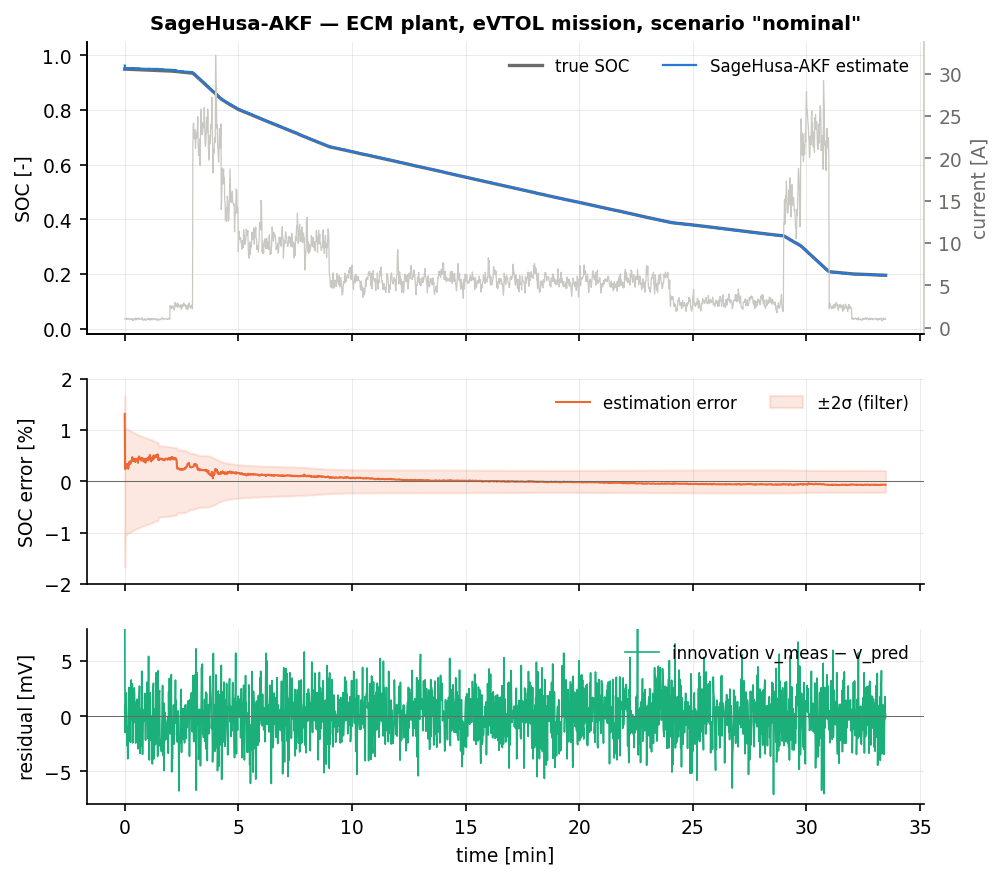
\includegraphics[width=\textwidth]{figures/cell_SageHusaAKF_nominal.png}
\caption{SageHusa-AKF on the nominal eVTOL mission: true and estimated SOC (top), estimation error with the $\pm 2\sigma$ band when available (middle), voltage residual (bottom).}
\end{figure}
\begin{figure}[H]\centering
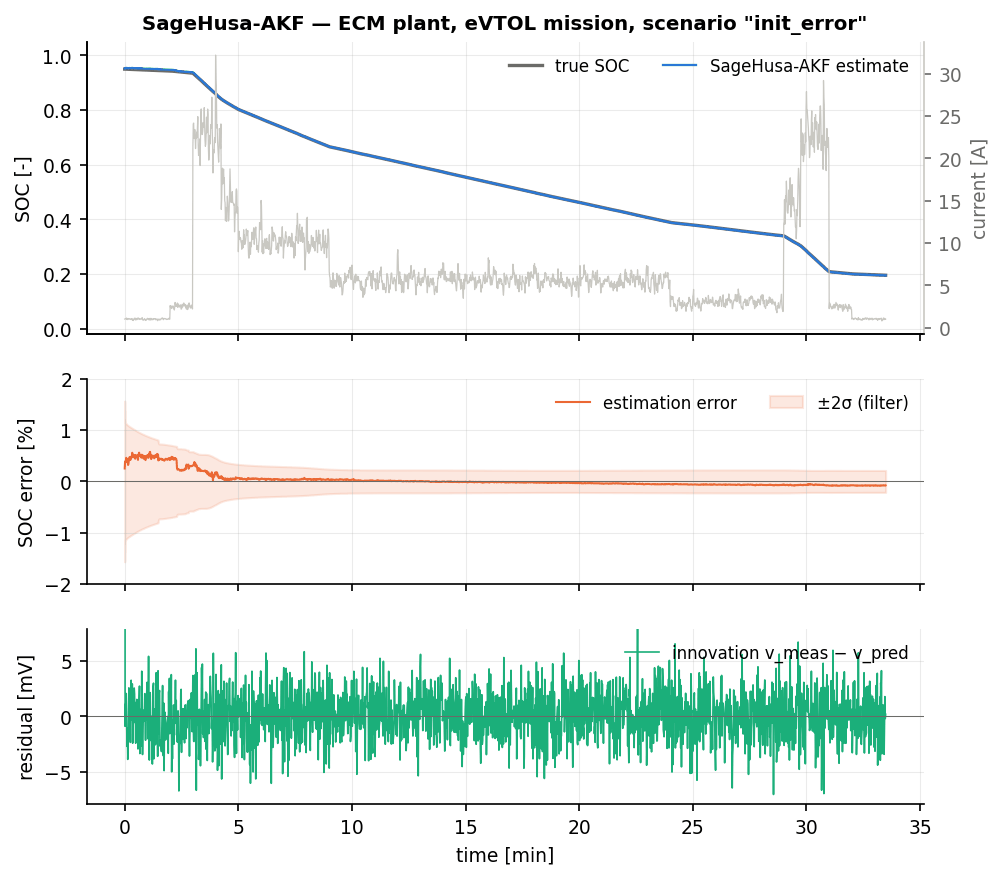
\includegraphics[width=\textwidth]{figures/cell_SageHusaAKF_init_error.png}
\caption{SageHusa-AKF with a 35\,\% initial SOC error.}
\end{figure}
\begin{figure}[H]\centering
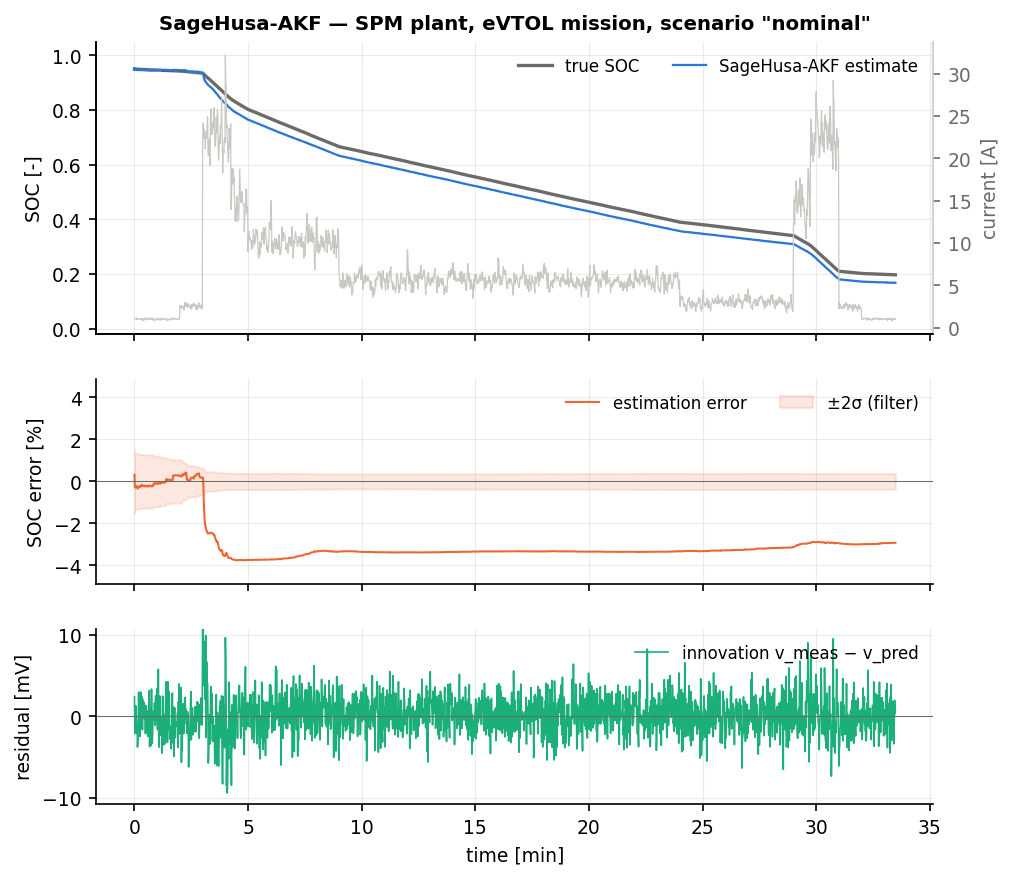
\includegraphics[width=\textwidth]{figures/cellspm_SageHusaAKF_nominal.png}
\caption{SageHusa-AKF on the electrochemical (single-particle) plant, nominal mission: the estimator uses a 2-RC ECM fitted to that plant and therefore sees a structured \SI{4}{\milli\volt} residual instead of white noise.}
\end{figure}

All figures below are three-seed means in \% SOC, as tabulated above; the plain \texttt{EKF} run on
the same data is the reference (\texttt{EKF ref.} column).  For orientation, the EKF scores
$\mathrm{rmse}_{ss}$ = 0.05\,\% on \texttt{nominal}, 0.12\,\% on \texttt{noise\_step}, 0.21\,\% on
\texttt{outliers}, 0.46\,\% on \texttt{sensor\_dropout}, 1.36\,\% on \texttt{param\_mismatch},
1.52\,\% on \texttt{aged\_cell} and 12.44\,\% on \texttt{combined} (where it never converges), and
3.73\,\% on the nominal SPM mission.

\paragraph{Benign scenarios.}  On \texttt{nominal} the filter matches the EKF and is marginally
better in steady state: $\mathrm{rmse}=0.24\,\%$, $\mathrm{rmse}_{ss}=\mathbf{0.04\,\%}$ against the
EKF's $0.15\,\%$ / $0.05\,\%$, both far inside the $2\,\%$ acceptance bound.  This is the expected
behaviour --- when the assumed $\mR$ is already correct, $\hat{\mR}_k$ fluctuates by $\pm10\,\%$
around it and the gain is unchanged.  On \texttt{init\_error} (35\,\% initial SOC error) the filter
converges within the first sample ($t_\mathrm{conv}=\SI{0}{\second}$, $\mathrm{rmse}=0.13\,\%$
against the EKF's $0.14\,\%$, maximum error $0.63\,\%$): the large prior covariance
$P_{0,\soc\soc}=\sigma_{z0}^2=0.01$ makes the first correction essentially a direct OCV inversion,
and the warm-up window prevents the corresponding \SI{30}{\milli\volt} residual from contaminating
$\hat{\mR}$.

\paragraph{Target scenario \texttt{noise\_step}.}  The voltage-sensor noise steps from
\SI{2}{\milli\volt} to \SI{20}{\milli\volt} at $t=\SI{600}{\second}$.  Measured on seed 1 and
averaged over $t\in[100,600)\,\si{\second}$ the filter reports
$\hat\sigma_v=\SI{2.17}{\milli\volt}$; over $t\in[700,2010]\,\si{\second}$ it reports
$\hat\sigma_v=\SI{19.99}{\milli\volt}$.  The identification is therefore essentially exact, and it
buys accuracy as well as consistency.  The EKF's steady-state SOC error rises from $0.05\,\%$ on
\texttt{nominal} to $0.12\,\%$ here, i.e.\ the tenfold sensor noise does leak into its SOC estimate
through a gain that is a factor $\sqrt{92}$ too large; the adaptive filter removes that leak
completely and returns to $\mathbf{0.04\,\%}$, a $3.0\times$ reduction.  Consistency is restored at
the same time: the normalised innovation squared $\mathrm{NIS}_k=\bm{e}_k^\T\mS_k\inv\bm{e}_k$, which
must average $n_y=1$ for a consistent filter, is $1.000$ before and $1.006$ after the step, whereas
the non-adaptive EKF goes from $1.099$ to $\mathbf{90.3}$ --- its innovations are a factor of
$\sqrt{90}\approx9.5$ larger than it believes, which would trip any residual-based fault monitor.
The voltage-prediction error falls accordingly, $\mathrm{rmse}_v$ from \SI{2.89}{\milli\volt} to
\SI{1.01}{\milli\volt}.

\paragraph{Where it wins on SOC.}  Adaptation pays wherever the innovations are inflated by something
the model cannot represent.  \texttt{sensor\_dropout} (the voltage reading freezes for
\SI{15}{\second} from $t=\SI{200}{\second}$): $\mathrm{rmse}$ $0.72\to0.23\,\%$ and
$\mathrm{rmse}_{ss}$ $0.46\to0.08\,\%$, factors of $3.1$ and $5.8$ --- the frozen sample stream
inflates the residuals, $\hat{\mR}$ grows, the gain collapses, and the filter coasts on coulomb
counting until the sensor recovers.  \texttt{param\_mismatch} ($R_0\times0.7$, $R_1\times1.3$,
$\tau_2\times1.5$): $1.28\to0.59\,\%$ and $1.36\to0.76\,\%$.  \texttt{outliers}:
$0.52\to0.22\,\%$ and $0.21\to0.06\,\%$ ($3.5\times$).  \texttt{aged\_cell}: $1.18\to1.07\,\%$ and
$1.52\to1.30\,\%$.  The largest effect is on \texttt{combined} (25\,\% initial SOC error,
\SI{150}{\milli\ampere} current bias, 2\,\% gain error, 10\,\% capacity loss), where the EKF
\emph{never} converges to the $2\,\%$ band ($t_\mathrm{conv}=$ --, $\mathrm{rmse}=16.02\,\%$,
$\mathrm{rmse}_{ss}=12.44\,\%$) while the Sage--Husa filter converges at $t=\SI{1446}{\second}$ with
$\mathrm{rmse}=4.95\,\%$ and $\mathrm{rmse}_{ss}=\mathbf{1.98\,\%}$ --- a $3.2\times$ and
$6.3\times$ reduction.  The mechanism is not the one the method was designed for: in
\texttt{combined} the cell's series resistance has grown to $1.25\,R_0$, which at the
\SI{5.5}{\ampere} cruise current is a \SI{16}{\milli\volt} bias on the predicted voltage; because the
NMC OCV curve is very flat near $\soc=0.9$ ($\partial\ocv/\partial\soc\approx\SI{0.2}{\volt}$ per
unit SOC), the EKF converts that bias into a $12\,\%$ SOC error.  Sage--Husa sees the bias as excess
measurement noise, inflates $\hat{\mR}$, and lets coulomb counting dominate --- which on this
scenario is the more accurate of the two information sources.

\paragraph{Costs and neutral cases.}  De-weighting the voltage channel is not free: $\mathrm{rmse}_v$
rises from \SI{3.80}{\milli\volt} to \SI{21.77}{\milli\volt} on \texttt{aged\_cell} and from
\SI{5.15}{\milli\volt} to \SI{13.91}{\milli\volt} on \texttt{combined}, because the filter
deliberately stops following a measurement it has decided is unreliable.  If the application needs an
accurate terminal-voltage prediction (for a power-limit computation, say) $\hat{\mR}$ must not be
allowed to grow without bound; \texttt{r\_max\_scale} is the knob.  On \texttt{cold}
($T=\SI{-10}{\celsius}$) the filter is slightly worse than the EKF ($0.22\,\%$ against $0.16\,\%$):
at low temperature the RC dynamics are slow, the residual sequence is strongly coloured, and that
violates \cref{as:sh:slow} and biases $\hat{\mR}$ upward.  On \texttt{preisach} --- the truth plant
uses a Preisach hysteresis operator with the corrected sign convention that the estimator does not
model --- the filter matches the EKF in steady state ($0.20\,\%$ for both) and is marginally worse
over the full run ($0.67\,\%$ against $0.58\,\%$), but it does reach the $2\,\%$ band immediately
($t_\mathrm{conv}=\SI{0}{\second}$ against the EKF's \SI{16}{\second}).  \texttt{current\_bias} is a
draw ($0.62\,\%$ against $0.61\,\%$): a constant current-sensor offset does not inflate the
innovations enough to trigger adaptation, and no amount of $\mR$ tuning can recover an input error.
Runtime is \SI{545}{\nano\second}/step against the EKF's \SI{478}{\nano\second}/step.

\paragraph{Electrochemical (SPM) plant.}  The SPM rows are the hard test: the estimator runs a 2-RC
ECM fitted to a single-particle model with Butler--Volmer kinetics and solid-diffusion time constant
$\tau\approx\SI{556}{\second}$, so the voltage residual is not white noise at all but a structured,
slowly varying \SI{4}{\milli\volt} signal.  Sage--Husa ends at $\mathrm{rmse}_{ss}=3.33\,\%$ on the
nominal SPM mission against the EKF's $3.73\,\%$ --- an improvement of barely $10\,\%$, and two
orders of magnitude worse than what the covariance-inflating filters achieve on the same data
(Fading-EKF $0.36\,\%$, STF $0.66\,\%$, \cref{ch:fadingekf} and \cref{ch:stf}).  The reason is
structural and is worth stating precisely, because it is the sharpest illustration in this chapter
of what covariance matching can and cannot do.  The recursion \eqref{eq:sh:Rrec} sees residuals that
are twice the nominal $\sigma_v$ and, being unable to ask \emph{why}, does the only thing it knows:
it raises $\hat{\mR}$ to about $(\SI{4}{\milli\volt})^2$ and lowers the Kalman gain.  Lowering the
gain hands the SOC estimate over to the coulomb integrator --- but on the SPM plant the integrator is
precisely the part that is wrong, because the fitted $Q_\mathrm{Ah}$ and coulombic efficiency do not
reproduce the true lithium inventory, so the estimate drifts to a $3\,\%$ offset and stays there.
The measurement, by contrast, is trustworthy: the ECM's static $\ocv(\soc)$ map \emph{was} fitted to
this plant, so the voltage still identifies SOC to a few tenths of a percent; what the ECM cannot
reproduce is the \emph{dynamics}.  Trusting the measurement more (inflating $\mP$) is therefore the
correct response and trusting it less (inflating $\mR$) is the wrong one, which is the exact mirror
image of the ECM \texttt{aged\_cell} result above, where the model error sat in the output equation
and inflating $\mR$ was right.  Where the SPM scenario adds an error \emph{on top of} the structural
one, the adaptation does earn its keep: \texttt{cold} $7.35\to2.65\,\%$ (a $2.8\times$ improvement,
the largest on the SPM plant) and \texttt{param\_mismatch} $3.13\to1.13\,\%$.  It is worse than the
EKF only on SPM \texttt{outliers} ($3.19\,\%$ against $1.99\,\%$), where inflating $\mR$ on top of an
already-conservative gain locks the estimate onto the drifting integrator.

\section{Summary}
The Sage--Husa filter is the cheapest useful adaptive Kalman filter: one extra output evaluation,
one $n_y\times n_y$ recursion, no inversion, no buffer.  Use it whenever the effective
measurement-noise level of a channel is uncertain or time-varying and you need the filter's
innovations to stay statistically consistent --- on this benchmark it tracks a tenfold voltage-noise
step to within $0.1\,\%$, holds $\overline{\mathrm{NIS}}\approx 1$ where the EKF reaches $90$, and
cuts the steady-state SOC error on that step from $0.12\,\%$ to $0.04\,\%$.
Do not use the $\mQ$ recursion: it is not identifiable jointly with $\mR$ and loses positive
definiteness.  Do not expect it to help when the residuals are inflated by structured model error rather than by
noise: on the electrochemical plant it improves on the EKF by barely $10\,\%$ ($3.33\,\%$ against
$3.73\,\%$) where the covariance-inflating filters reach $0.36\,\%$, because lowering the gain is
the wrong response when the model, not the sensor, is the unreliable component.  It cannot
distinguish a noisy sensor from a wrong model --- when the two must be told apart, use the IMM
(\cref{ch:imm}) instead.
